\section{Task4: Implementation– Sprint 1}
\subsection{Setting up an online repository github for version control}
Link GitHub của nhóm: https://github.com/TitaniumBull224/se-ssps 
\subsection{Add Requirements, Modeling, and Design files to GitHub with version control.}
\begin{figure}[htbp]
    \centering
    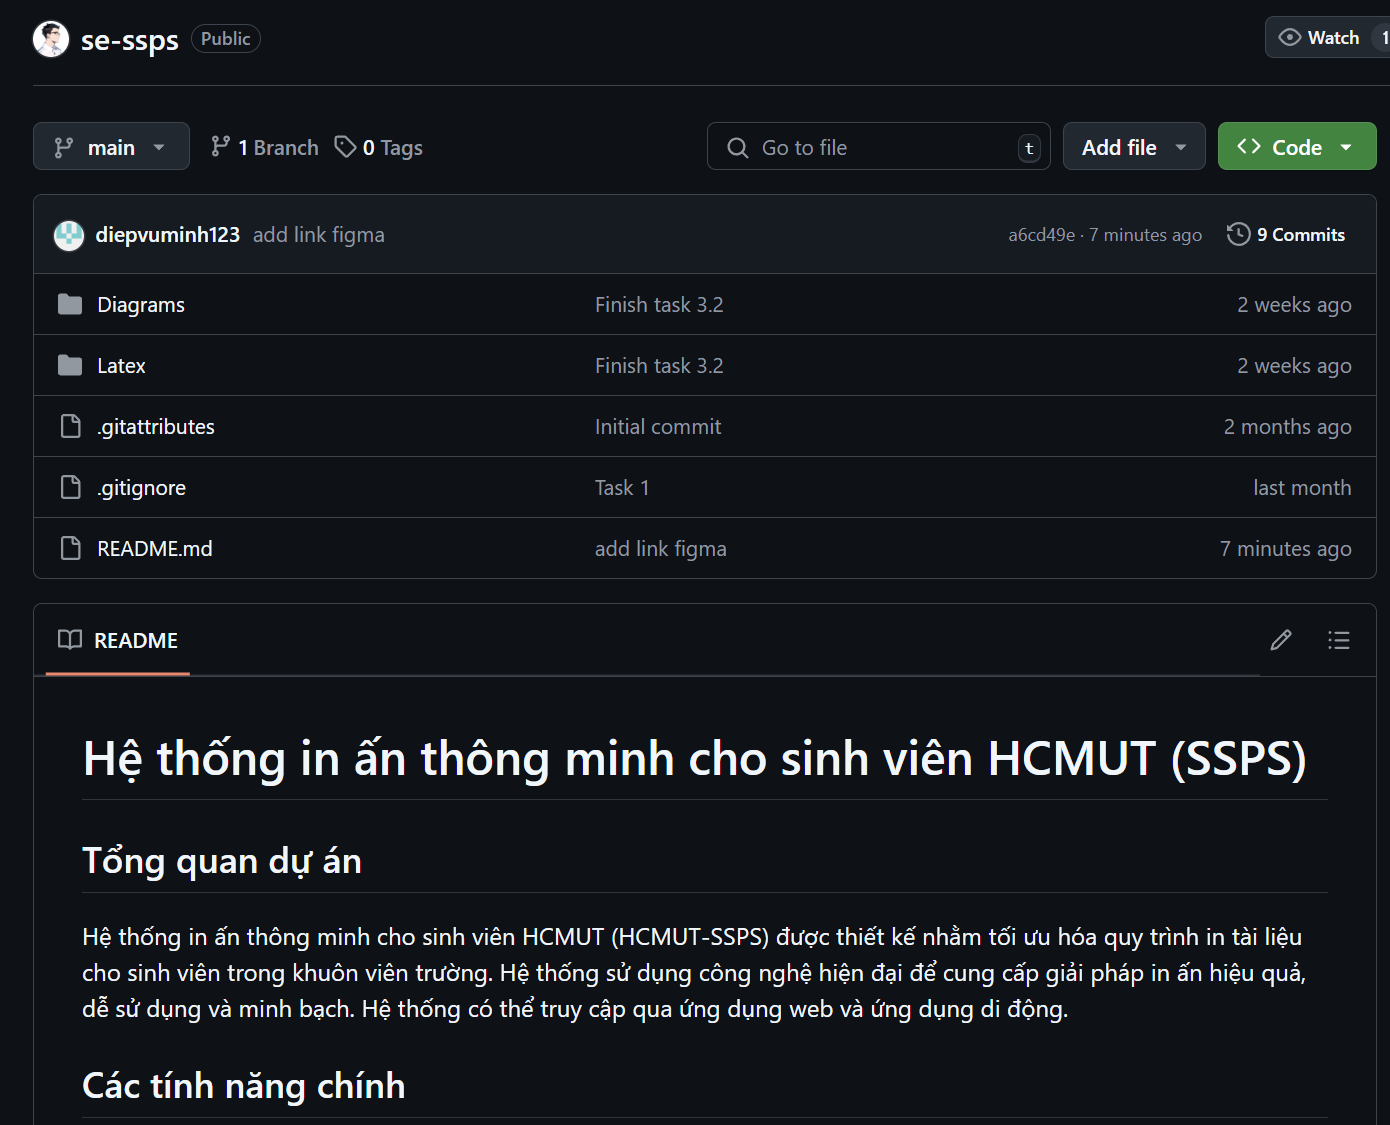
\includegraphics[width=1\linewidth]{Images/Github.png}
    \caption{Repository GitHub}
\end{figure}
\subsection{Usability test}

\begin{itemize}
    \item \textbf{Bước 1}: Chọn/Tìm testers để thực hiện usability test \\ 
    Nhóm đã tìm được 3 tester và tester yêu cầu giấu kín thông tin cá nhân của họ.
    \item \textbf{Bước 2}: Thiết kế các tác vụ mà Tester sẽ thực hiện trên ứng dụng\\
    Các tác vụ mà tester sẽ thực hiện là:
    \begin{itemize}
        \item Sinh viên xem lịch sử in
        \begin{enumerate}
            \item Tại giao diện chính của sinh viên, Tester bấm vào mục xem lịch sử in
            \item Hệ thống sẽ hiện thị lịch sử in.
        \end{enumerate}
        \item Sinh viên xem bảng điều khiển.
        \item Sinh viên tải tài liệu và điều chỉnh hệ thống in
        \item SPSO quản lý máy in 
        \begin{enumerate}
            \item Tại giao diện của SPSO, bấm vào mục "Quản lý máy in" trên thanh tác vụ
            \item Giao diện sẽ ra danh sách chi tiết các máy in có trong hệ thống
        \end{enumerate}
        \item SPSO xem lịch sử in của sinh viên.
        \begin{enumerate}
            \item Tại giao diện của SPSO, bấm vào mục "Xem lịch sử" trên thanh tác vụ
            \item Giao diện sẽ ra bản lưu chi tiết lịch sử in đã được thực hiện trên tất cả các máy in thuộc hệ thống 
        \end{enumerate}
    \end{itemize}
     \newpage
    Các test-case:
    \begin{longtable}{|l|c|}
        \hline
        \textbf{Test case} & Xem lịch sử in \\
        \hline
        \textbf{Test description} & Sinh viên xem lịch sử in \\
        \hline
        \textbf{Pre-condition} & User đăng nhập với tư cách student và đang ở trang chính \\
        \hline
        \textbf{Actions} & 1. Người dùng bấm vào xem lịch sử in \\
        \hline
        \textbf{Expected outputs} & Màn hình hiện thị lịch sử in của sinh viên\\
        \hline
    \end{longtable}
    
    \begin{longtable}{|l|p{9cm}|} 
    \hline
    \textbf{Test case} & Xem bảng điều khiển \\
    \hline
    \textbf{Test description} & Sinh viên xem giao diện chính của Bảng điều khiển \\
    \hline
    \textbf{Pre-condition} & User đã đăng nhập với tư cách sinh viên \\
    \hline
    \textbf{Actions} & 1. Người dùng đăng nhập thành công và được chuyển đến trang Bảng điều khiển \\
    \hline
    \textbf{Expected outputs} & 
    \parbox[t]{9cm}{
        Màn hình hiển thị các thông tin sau:
        \begin{itemize}
            \item Ảnh đại diện, tên, ngành học, mã sinh viên.
            \item Các mục chính: Lịch sử in, Số trang in còn lại, và danh sách các hoạt động gần đây.
        \end{itemize}
    } \\
    \hline
    \end{longtable}
    
    \begin{longtable}{|l|p{9cm}|} 
    \hline
    \textbf{Test case} & Tải tài liệu và điều chỉnh hệ thống  \\
    \hline
    \textbf{Test description} & Sinh viên tải tài liệu và tùy chỉnh cài đặt in tài liệu \\
    \hline
    \textbf{Pre-condition} & 
    User đã đăng nhập thành công vào hệ thống với tư cách sinh viên.\newline
    User truy cập vào mục "In tài liệu".\\
    \hline
    \textbf{Actions} & 
    1. Người dùng chọn tài liệu muốn in. \newline
    2. Người dùng điều chỉnh các tùy chọn trong phần Cài đặt in(Chọn máy in, số bản in,...)
    3. Nhấn nút In để thực hiện in tài liệu. \\
    \hline
    \textbf{Expected outputs} & 
    \parbox[t]{9cm}{       
    Khi nhấn nút In, một trong các kết quả sau xảy ra:
    \begin{itemize}
        \item In thành công: Tài liệu được gửi đến máy in với cài đặt đã chọn.
        \item Lỗi thông báo: Nếu gặp lỗi như máy in không kết nối, giấy không đủ, hoặc trang in không tồn tại, hệ thống hiển thị thông báo lỗi chi tiết.
    \end{itemize}
    } \\
    \hline
    \end{longtable}
    
    \item \textbf{Bước 3}: Chọn phương pháp Test \\
    Phương pháp test là remote.
    \item \textbf{Bước 4}: Tiến hành test
    \item \textbf{Bước 5}: Nhận feedback từ các tester\\
    Tester 1 nhận xét về xem lịch sử in của student:  
    \begin{enumerate}
    \item \textbf{Giao diện thân thiện:} 
    \begin{itemize}
        \item Giao diện của hệ thống đẹp mắt,rõ ràng và dễ sử dụng. 
        \item Thanh tìm kiếm được đặt ở vị trí dễ thấy và có thể hỗ trợ tìm kiếm nhanh chóng.
    \end{itemize}

    \item \textbf{Cột thông tin đầy đủ:}
    \begin{itemize}
        \item Các thông tin như số thứ tự, tên file, số tờ, thời gian và máy in đều được hiển thị rõ ràng và đầy đủ.
        \item Điều này giúp dễ dàng theo dõi các lệnh in đã thực hiện.
    \end{itemize}

    \item \textbf{Trải nghiệm tổng thể:}
    \begin{itemize}
        \item \textbf{Điểm tốt:} Tốc độ tải dữ liệu nhanh, không bị giật lag. Việc phân trang cũng rõ ràng và dễ thao tác.
        \item \textbf{Cần cải thiện:}
        \begin{itemize}
            \item Hiện tại, tên file được lặp lại quá nhiều. Nếu có cách để nhóm các lệnh in trùng lặp hoặc thêm các tùy chọn lọc nâng cao, như lọc theo thời gian hoặc tên file, sẽ cải thiện đáng kể trải nghiệm.
            \item Hệ thống chưa cung cấp trạng thái chi tiết của lệnh in, ví dụ: ``Đang chờ'', ``Đã hoàn thành'', hoặc ``Lỗi''. Thông tin này rất hữu ích nếu gặp sự cố.
            \item Hình ảnh máy in hoặc biểu tượng tương ứng có thể làm giao diện sinh động hơn.
        \end{itemize}
    \end{itemize}

    \item \textbf{Khả năng mở rộng:}
    \begin{itemize}
        \item Hy vọng hệ thống có thể hỗ trợ thêm các tính năng như tải xuống lịch sử in dưới dạng file Excel hoặc PDF để dễ dàng lưu trữ.
    \end{itemize}
\end{enumerate}
  Tester 2 nhận xét về Bảng điều khiển và In tài liệu:
  \begin{enumerate}
      \item \textbf{Tải tài liệu và Điều chỉnh hệ thống in}
      \begin{itemize}
          \item Điểm tốt:
          \begin{itemize}
              \item Giao diện được thiết kế hợp lý với các phần chính như xem trước tài liệu, cài đặt in, và nút hành động được sắp xếp khoa học, giúp người dùng dễ dàng thao tác.
              \item Người dùng có thể điều chỉnh nhiều thiết lập quan trọng như khổ giấy, hướng giấy, số trang cụ thể, và số bản in. Điều này tăng tính linh hoạt khi sử dụng.
              \item Chức năng xem trước tài liệu giúp người dùng kiểm tra nội dung trước khi in, giảm nguy cơ sai sót.
          \end{itemize}
          \item Cần cải thiện:
          \begin{itemize}
              \item Thêm các hướng dẫn ngắn hoặc tooltip cho các thao tác phức tạp (ví dụ: “Sử dụng dấu phẩy để chọn các trang cụ thể: 1-3,5”).
          \end{itemize}
      \end{itemize}
      \item \textbf{Bảng điều khiển:}
      \begin{itemize}
          \item Điểm tốt:
          \begin{itemize}
              \item Trang hiển thị rõ ràng các thông tin cá nhân của người dùng (ảnh đại diện, tên, ngành học, mã sinh viên) cùng với số trang in còn lại và lịch sử in gần đây.
              \item Phần "Gần đây" giúp người dùng theo dõi chi tiết các lần in trước, bao gồm trạng thái thành công hay thất bại.
              \item Các nút truy cập nhanh (như “Xem lịch sử in”) giúp thao tác thuận tiện hơn.
          \end{itemize}
          \item Khả năng mở rộng:
          \begin{itemize}
              \item Cung cấp dự đoán về số trang in còn lại dựa trên tốc độ sử dụng gần đây, giúp người dùng lên kế hoạch mua thêm trang in khi cần thiết.
          \end{itemize}
      \end{itemize}
      
  \end{enumerate}
  Tester 3 nhận xét về "Quản lý máy in" và "xem lịch sử in của sinh viên" của SPSO \\
  \begin{enumerate}
      \item \textbf{SPSO quản lý máy in}
      \begin{itemize}
          \item Giao diện "Quản lý sinh viên" của SPSO hiển thị đầy đủ thông tin về các máy in, bao gồm tên máy, mô tả, trạng thái, và vị trí cụ thể của máy (cơ sở, tòa nhà, phòng). Giao diện có chữ dễ đọc, hỗ trợ sắp xếp hoặc lọc theo từng mục, có chức năng tìm kiếm máy in theo tên và mục "Thêm máy in" nằm ở vị trí thuận mắt.
      \end{itemize}
      
      \item \textbf{SPSO xem lịch sử in của sinh viên}
      \begin{itemize}
          \item Giao diện "Xem lịch sử" hiển thị đầy đủ thông tin lịch sử in gồm thông tin sinh viên (Họ và tên, MSSV), tên chủ đề, số bản in, thời gian in (ngày và giờ) và tên máy in được sử dung. Chữ trên giao diện được thiết kế dễ đọc, hỗ trợ sắp xếp theo từng mục, có chức năng tìm kiếm lịch sử in theo tên hoặc MSSV của sinh viên.
      \end{itemize}
  \end{enumerate}

\end{itemize}
